% Author: Alex Tsolovikos

\documentclass[18pt,xcolor=table]{beamer}

\usepackage{bbm}
\usepackage{textpos}

% \definecolor{utorange}{RGB}{203,96,21}
\definecolor{utorange}{RGB}{191,87,0}
% \definecolor{utblack}{RGB}{99,102,106}
\definecolor{utblack}{RGB}{51,63,72}
\definecolor{utbrown}{RGB}{110,98,89}
\definecolor{utsecbrown}{RGB}{217,200,158}
\definecolor{utsecgreen}{RGB}{208,222,187}
\definecolor{utsecblue}{RGB}{127,169,174}
\definecolor{utsectan}{RGB}{248,151,31}
\definecolor{utseclimestone}{RGB}{214,210,196}

\mode<presentation>
{   
    \usetheme{Boadilla}  

    \usefonttheme[onlymath]{serif}

    \setbeamercovered{invisible}
    \setbeamertemplate{navigation symbols}{}
    
    % Color Theme 
    \setbeamercolor{normal text}{bg=white,fg=utblack} % Main body text color
    \setbeamercolor{structure}{fg=utblack} % Slide title color
    \setbeamercolor{alerted text}{fg=red!85!black}
    \setbeamercolor{item projected}{use=item,fg=black,bg=item.fg!35}
    \setbeamertemplate{enumerate item}{\insertenumlabel.}
    \setbeamertemplate{itemize items}[circle]
    \setbeamertemplate{itemize subitem}{{\textendash}}
    \setbeamercolor{subitem}{fg=utblack}
    
    % Burnt-orange footnote bar
    \setbeamercolor*{palette primary}{use=structure,fg=white, bg=utorange}
    \setbeamercolor*{palette secondary}{use=structure,fg=white,bg=utorange}
    \setbeamercolor*{palette tertiary}{use=structure,fg=white,bg=utorange}

    \setbeamercolor*{palette quaternary}{use=structure,fg=structure.fg,bg=utsecblue}
    
    \setbeamercolor*{framesubtitle}{fg=utblack}
    
    \setbeamercolor*{block title}{parent=structure,fg=black,bg=utseclimestone}
    \setbeamercolor*{block body}{fg=black,bg=utblack!10}
    \setbeamercolor*{block title alerted}{parent=alerted text,bg=black!15}
    \setbeamercolor*{block title example}{parent=example text,bg=black!15}
    
    \setbeamerfont{framesubtitle}{size=\small}
    \setbeamerfont{author1}{size=\small}
}

\pgfdeclareimage[height=1.6cm]{asebig}{figs/Cockrell_RGB_formal_ASE_EM}

\usepackage[orientation=landscape,size=custom,width=16,height=9.75,scale=0.5,debug]{beamerposter}

\addtobeamertemplate{footnote}{\vspace{-6pt}\advance\hsize-0.5cm}{\vspace{6pt}}
\makeatletter

% Alternative A: footnote rule
\renewcommand*{\footnoterule}{\kern -3pt \hrule \@width 2in \kern 8.6pt}

% Alternative B: no footnote rule
% \renewcommand*{\footnoterule}{\kern 6pt}

\makeatother

% Footer
\makeatletter
\setbeamertemplate{footline}
{
\leavevmode%
    \hbox{%
        \begin{beamercolorbox}[wd=\paperwidth,ht=2.25ex,dp=1ex,center]{author in head/foot}%
            \centering%
            \hspace*{2ex}
            \usebeamerfont{author in head/foot} \insertshortauthor%
            \hfill%
            \usebeamerfont{title in head/foot}\insertshorttitle%
            \hfill%
            \usebeamerfont{date in head/foot}\insertshortdate{}%
            \hfill%
            \insertframenumber{} / \inserttotalframenumber\hspace*{2ex} 
        \end{beamercolorbox}%
    }%
}
\makeatother

% At the beginning of each section
\AtBeginSection[]{
    \begin{frame}
        % \vfill    
        \centering
        \begin{beamercolorbox}[sep=8pt,center,rounded=true]{title}
            % \vspace*{2cm}%
            \usebeamerfont{title}\insertsectionhead\par%
        \end{beamercolorbox}
%   \rule{11cm}{0.4pt}\par
        % \vfill
    \end{frame}
}


\makeatletter
    \DeclareMathSizes{\f@size}{2}{2}{2}
\makeatother

\renewcommand*{\thefootnote}{\fnsymbol{footnote}}

\newcommand{\foo}{\color{utorange}\makebox[0pt]{\textbullet}\hskip-0.5pt\vrule width 1pt\hspace{\labelsep}}


%Create Last Page
\newcommand{\lastframe}{%
\begin{frame}
    \centering
    \vspace{1cm}
    \pgfuseimage{asebig}
\end{frame}
}

% -----------------------------------------------------------------------------------
% Insert your title info here
% -----------------------------------------------------------------------------------
\title[Short Title]{The Greatest Presentation Ever}
\author[First Last Name, The University of Texas at Austin]{First Name Last Name}

\institute{
    Department of Aerospace Engineering and Engineering Mechanics \\ 
    The University of Texas at Austin \\ 
}
\institute{Graduate Student \\Aerospace Engineering and Engineering Mechanics \\ The University of Texas at Austin}
\date[June 2022, Austin, TX]{Austin, TX, June 2022}

% -----------------------------------------------------------------------------------
% Other Packages
% -----------------------------------------------------------------------------------

\usepackage{hyperref}
\usepackage{amsmath,amsfonts,amssymb}
\usepackage{color}
\usepackage{caption}
\usepackage{subcaption}
\usepackage{graphics} % for pdf, bitmapped graphics files
\usepackage{epsfig} % for postscript graphics files
\usepackage{mathtools}% http://ctan.org/pkg/mathtools
\usepackage{animate}
\usepackage{tabularx}
\usepackage{bigdelim}
\usepackage{bm}
\usepackage[style=verbose]{biblatex}

%Add bibliography file location for citations
\bibliography{biblio.bib}

%Enable cancelto in math
\usepackage{cancel}
\renewcommand{\CancelColor}{\color{utorange}}

% -----------------------------------------------------------------------------------
  
\begin{document}

% -----------------------------------------------------------------------------------
% Title frame
% -----------------------------------------------------------------------------------

{ % Define the headline only for the first slide
\makeatletter
\setbeamertemplate{headline}
{
\leavevmode%
    \hbox{%
        \begin{beamercolorbox}[wd=\paperwidth,ht=0.9cm,dp=1ex,center]{author in head/foot}%
            % \begin{flushleft}
            % \includegraphics[width=0.95\paperwidth]{figs/ASE_UT_Header_Logo_Beamer.eps}%
            \begin{columns}
            \begin{column}{0.01\paperwidth}
            \end{column}
            \begin{column}{0.4\paperwidth}
                \vspace{-1.05cm}
                \begin{flushleft}
                
\includegraphics[height=0.85cm]{figs/Cockrell_KO_formal_ASE_EM.png}%                
                \end{flushleft}
            \end{column}%
            \begin{column}{0.5\paperwidth}
                \vspace{-1.05cm}
                \begin{flushright}
                 
\includegraphics[height=2cm]{figs/utexas.png}%                
                \end{flushright}
            \end{column}
            \end{columns}
            % 
\includegraphics[height=0.85cm]{figs/Cockrell_KO_formal_ASE_EM.png}%
            % \end{flushleft}
        \end{beamercolorbox}%
    }%
}
\makeatother

\setbeamertemplate{headline}[miniframes theme]
\frame{\titlepage}
}

% -----------------------------------------------------------------------------------

\begin{frame}
    \frametitle{Slide with Text and Image}
    \begin{columns}
    \begin{column}{0.4\linewidth}
        \begin{itemize}
            \item List item 1
            \item List item 2
            \item List item 3
        \end{itemize}
    \end{column}%
    \begin{column}{0.6\linewidth}
        \centering
        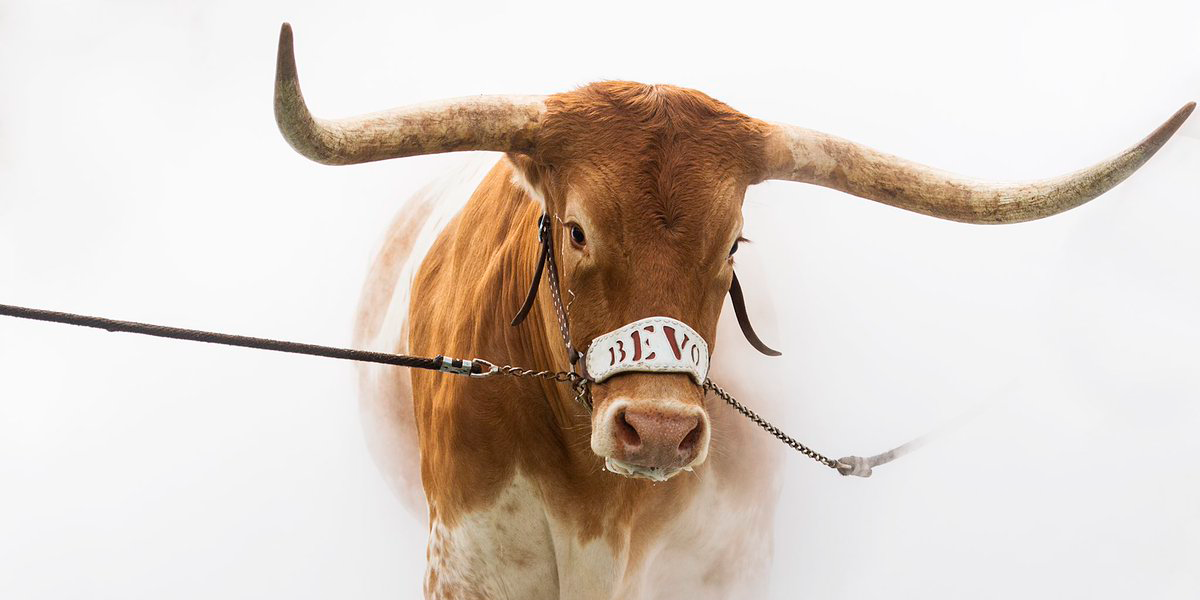
\includegraphics[scale=0.2]{figs/bevo.png}
    \end{column}
    \end{columns}
\end{frame}

% -----------------------------------------------------------------------------------

\section{Main Section} % Adds a section slide

% -----------------------------------------------------------------------------------

\begin{frame}
    \frametitle{One Column Slide}
    \begin{columns}
    \begin{column}[t]{\linewidth}
        {\footnotesize
        $$
            a(x_1,x_2) \frac{\partial^2 u}{\partial x_1^2} + b(x_1,x_2) \frac{\partial^2 u}{\partial x_1\partial x_2} +
            c(x_1,x_2) \frac{\partial^2 u}{\partial x_2^2} + d(x_1,x_2) \frac{\partial u}{\partial x_1} +
            e(x_1,x_2) \frac{\partial u}{\partial x_2} + f(x_1,x_2) u = g(x_1,x_2)
        $$
        }
        \begin{itemize}
            \item {The PDE is called ``elliptic'' if
                $$
                     {
                     b^2 - 4ac < 0
                     }
                $$}
            \item {The PDE is called ``hyperbolic'' if
                $$
                     {
                     b^2 - 4ac > 0
                     }
                $$}
            \item {The PDE is called ``parabolic'' if
                $$
                     {
                     b^2 - 4ac = 0
                     }
                $$}
        \end{itemize}
    \end{column}
    \end{columns}
\end{frame}

% -----------------------------------------------------------------------------------

\begin{frame}
    \frametitle{Slide with Two Columns\footcite{rasmussen2003gaussian}}
    \begin{columns}
    \begin{column}{0.5\linewidth}
        \begin{itemize}
            \item List item 1
            \item List item 2 with \textcolor{utorange}{equation} $$f(\cdot) : \Rb^n \rightarrow \Rb$$
            \item Sublist:
            \begin{itemize}
                \item One
                \item Two
                \item Three
            \end{itemize}
        \end{itemize}
    \end{column}%
    \begin{column}{0.5\linewidth}
        \begin{itemize}
            \item List item 1
            \item List item 2 with \textcolor{utorange}{equation} $$f(\cdot) : \Rb^n \rightarrow \Rb$$
            \item Sublist:
            \begin{itemize}
                \item One
                \item Two
                \item Three
            \end{itemize}
        \end{itemize}
    \end{column}
    \end{columns}
\end{frame}

% -----------------------------------------------------------------------------------

\begin{frame}
    \frametitle{Conclusion and Future Work}
    \begin{columns}
    \begin{column}{0.5\linewidth}
        \begin{itemize}
            \item I did this
            \item I did that
            \item Next steps:
            \begin{itemize}
                \item I will do A
                \item I will also do B
            \end{itemize}
        \end{itemize}
    \end{column}%
    \begin{column}{0.5\linewidth}
        \centering
        
\includegraphics[scale=0.8]{figs/ut_tower.png}
    \end{column}
    \end{columns}
    \vspace{0.5cm}
    \begin{block}{My Main Point}
        This is an emphasized text box.
    \end{block}
\end{frame}

% -----------------------------------------------------------------------------------
% If you want to customize the last frame, uncomment the following
% -----------------------------------------------------------------------------------

% { % Add the header back for the last slide
%     \makeatletter
%     \setbeamertemplate{headline}
%     {
%     \leavevmode%
%         \hbox{%
%             \begin{beamercolorbox}[wd=\paperwidth,ht=0.9cm,dp=1ex,center]{author in head/foot}%
%                 \centering
%                 \vspace*{-0.05cm}
%                 \includegraphics[width=0.95\paperwidth]{figs/ASE_UT_Header_Logo_Beamer.eps}%
%             \end{beamercolorbox}%
%         }%
%     }
%     \makeatother
    
%     \setbeamertemplate{headline}[miniframes theme]
    
%     % Now, write the last frame
%     \begin{frame}
%         \centering
%         \vspace{3cm}
%         \begin{figure}
%             \centering
%             \begin{subfigure}[c]{\textwidth}
%                 \centering
%                 
\includegraphics[scale=0.5]{figs/Cockrell_RGB_formal_ASE_EM.png}
%             \end{subfigure}
%         \end{figure}
%         \vspace{1.5cm}
%     \end{frame}
% }

% -----------------------------------------------------------------------------------

\lastframe

% -----------------------------------------------------------------------------------

\end{document}
